\section{Exact Projection}

\begin{frame}[t]\frametitle{Exact Projection}

  \begin{definition}[2.1]
    The \textcolor{purple}{exact  projection} of the point $v\in \mathbb{R}^{n}$ onto $C$ with respect to the norm $\| \cdot \| _{D}$, denoted by  ${\cal P}_{C}^{D}(v)$, is  defined~by
    \begin{equation*}
      {\cal P}_{C}^{D}(v):=\arg \min _{z\in C}\|z-v\|^2_{D}.
    \end{equation*}
  \end{definition}

  \bigskip
  \bigskip
  \bigskip

  \begin{lemma}[2.2]
    Let $v, w \in {\mathbb R}^n$.  Then,  $w={\cal P}_{C}^{D}(v)$ if and only if  $w\in C$ and
    \[
      \left\langle D(v-w), y-w\right\rangle \leq  0,
    \]
    for all $y \in C.$
  \end{lemma}
\end{frame}

\begin{frame}[t]\frametitle{Exact Projection}\bigskip
  \begin{figure}[!ht]
    \centering
    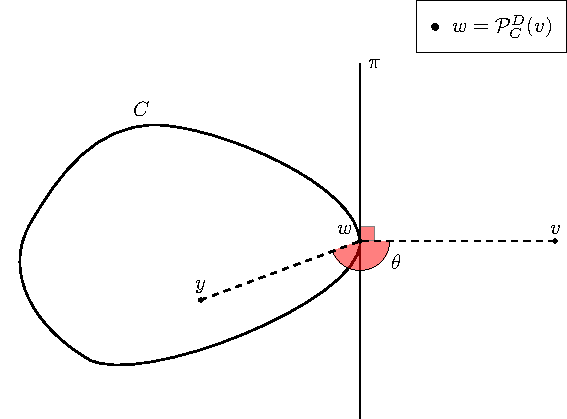
\includegraphics{../figures/exactProj.pdf}
    \caption{Exact projection of the point $v$ onto $C$.}
    \label{fig:exactProj}
  \end{figure}
\end{frame}

\section{Inexact Projections}


\begin{frame}
  \frametitle{Inexact Projections}

  \begin{definition}[2.5\footfullcite{BirginMartinezRaydan2003}]
    The feasible inexact projection mapping, with respect to the norm $\| \cdot \|_{D}$,   onto $C$  relative to a point  $u \in C$ and forcing parameter $\zeta\in (0, 1]$, denoted by ${\cal P}_{C,\zeta}^{D}(u,  \cdot): {\mathbb R}^n \rightrightarrows C$,  is the set-valued mapping defined as follows
    \begin{equation*}
      {\cal P}_{C,\zeta}^{D}(u, v) := \left\{w\in C:~ \|w-v\|_{D}^2\leq \zeta \| {\cal P}_{C}^{D}(v)-v\|_{D}^2+(1-\zeta)\|u-v\|_{D}^2 \right\}.
    \end{equation*}
    Each point $w\in {\cal P}_{C,\zeta}^{D}(u, v) $ is called a  \textcolor{purple}{feasible inexact projection},  with respect to the norm $\| \cdot \|_{D}$,  of $v$ onto $C$ relative to $u$ and forcing parameter $\zeta\in (0, 1]$.
  \end{definition}
\end{frame}

\begin{frame}[t]\frametitle{Inexact Projections}\bigskip
  \begin{figure}[H]
    \centering
    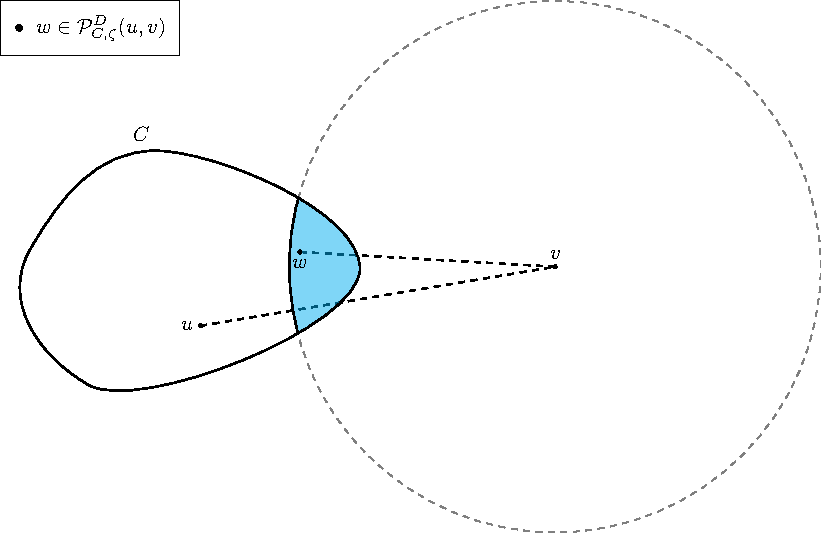
\includegraphics[height=0.725\textheight]{../figures/martinezProj.pdf}
    \caption{Feasible inexact projection of the point $v$ onto $C$.}
    \label{fig:martinezProj}
  \end{figure}
\end{frame}


\begin{frame}[t]\frametitle{Inexact Projections}
  \begin{definition}[2.10\footfullcite{SalzoVilla2012}\footfullcite{OrizonFabianaGilson2018}]
    The feasible inexact projection mapping, with respect to the norm $\| \cdot \|_{D}$,  onto $C$ relative to $u \in C$ and forcing parameter $\gamma\geq 0$, denoted by ${\cal R}_{C,\gamma}^{D}(u, \cdot): {\mathbb R}^n \rightrightarrows C$,  is the set-valued mapping defined as follows
    \begin{equation*}
      {\cal R}_{C,\gamma}^{D}(u, v):= \left\{w\in C:~\left\langle D(v-w), y-w \right\rangle \leq \gamma \|w-u\|_{D}^2, \quad \forall~ y \in C \right\}.
    \end{equation*}
    Each point $w\in {\cal R}_{C,\gamma}^{D}(u, v)$ is called a \textcolor{purple}{feasible inexact projection},  with respect to the norm $\| \cdot \|_{D}$,  of $v$ onto $C$ relative to $u$ and forcing parameter $\gamma\geq 0$.
  \end{definition}
\end{frame}


\begin{frame}[t]\frametitle{Inexact Projections}
  Let $u\in C$, $v\in \mathbb{R}^n$, $w\in{\cal R}_{C,\gamma}^{D}(u, v)$ be as stated in Definition 2.10, $0\leq t <1$ and
  $$
    w_t = w+t(v-w).
  $$
  Since
  $$
    \left\langle D(v-w), y-w \right\rangle \leq \gamma \|w-u\|_{D}^2,
  $$
  for all $y\in C$ we have
  \begin{align*}
    \begin{aligned}
      \left\langle D(v-w_t), y-w_t \right\rangle & \leq  (1-t)\left[ \gamma \|w-u\|_D^2 - t\|v-w\|_D^2 \right].
    \end{aligned}
  \end{align*}

  It follows that, for all
  \begin{equation}
    t \geq \frac{\gamma \|w-u\|_D^2}{\|v-w\|_D^2}
  \end{equation}
  $w_t$ satisfies
  \begin{equation}
    \left\langle D(v-w_t), y-w_t \right\rangle\leq 0.
  \end{equation}
\end{frame}


% \begin{frame}[t]\frametitle{Inexact Projections}\bigskip   
%   \begin{figure}[H]
%   %\begin{adjustwidth}{2.2cm}{2.2cm}
%   \begin{subfigmatrix}{2}
%     \subfigure[Geometric interpretation.]{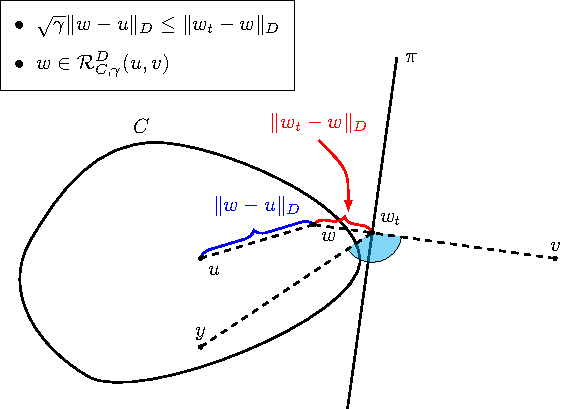
\includegraphics{../figures/condProj1.pdf}}
%     \subfigure[Example of ${\cal R}_{C,\gamma}^{D}(u, v)$.]{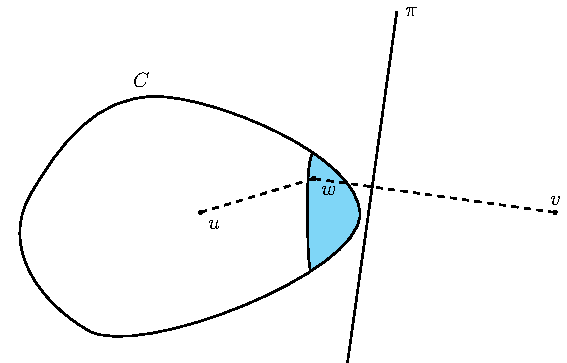
\includegraphics{../figures/condProj2.pdf}}
%   \end{subfigmatrix}
%   \caption{Geometric interpretation of projection ${\cal R}_{C,\gamma}^{D}(u, v)$.}
%   \label{fig:condProj1}
%   %\end{adjustwidth}
% \end{figure}
% \end{frame}

% \begin{frame}[t]\frametitle{Inexact Projections}\bigskip   
% \begin{figure}[H]
%   %\begin{adjustwidth}{2.2cm}{2.2cm}
%   \begin{subfigmatrix}{3}
%     \subfigure[]{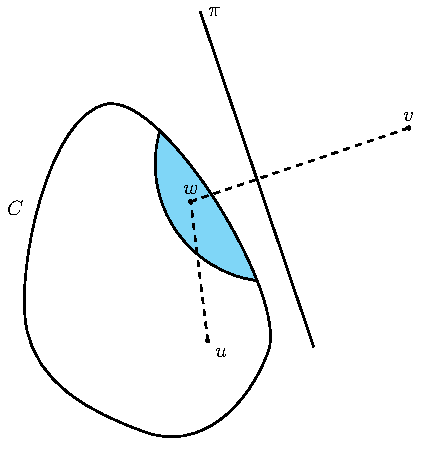
\includegraphics{../figures/condProj3.pdf}}
%     \subfigure[]{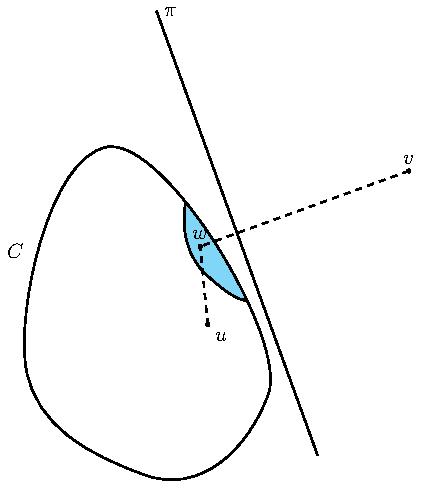
\includegraphics{../figures/condProj4.pdf}}
%     \subfigure[]{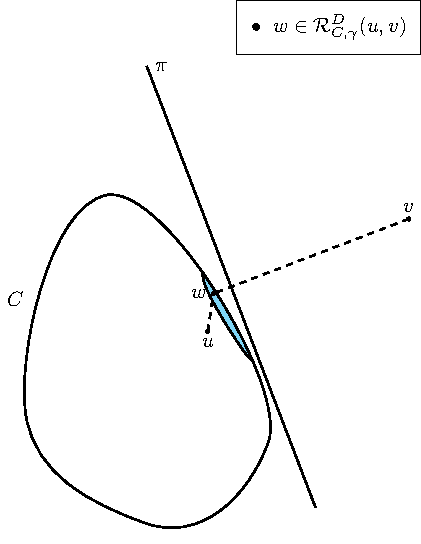
\includegraphics{../figures/condProj5.pdf}}
%   \end{subfigmatrix}
%   \caption{Examples of regions given by inexact projection ${\cal R}_{C,\gamma}^{D}(u, v)$.}
%   \label{fig:baseline}
%   %\end{adjustwidth}
% \end{figure}
% \end{frame}

% \begin{frame}[t]\frametitle{Inexact Projections}\bigskip   
% \begin{figure}[H]
%   \begin{subfigmatrix}{3}
%     \subfigure[]{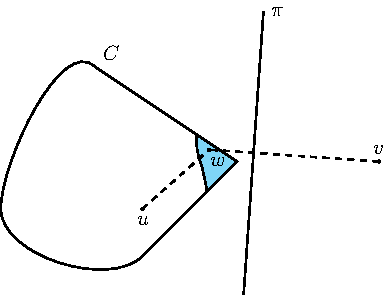
\includegraphics[width=0.3\textwidth]{../figures/condProj6.pdf}}
%     \subfigure[]{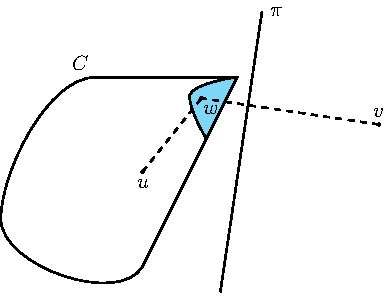
\includegraphics[width=0.3\textwidth]{../figures/condProj7.pdf}}
%     \subfigure[]{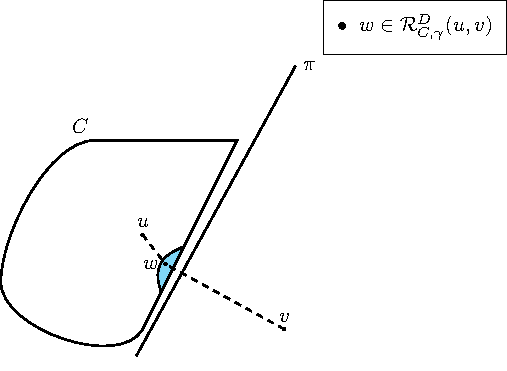
\includegraphics[width=0.37\textwidth]{../figures/condProj8.pdf}}
%   \end{subfigmatrix}
%   \caption{Examples of regions given by inexact projection ${\cal R}_{C,\gamma}^{D}(u, v)$.}
%   \label{fig:baseline}
% \end{figure}
% \end{frame}


\begin{frame}[t]\frametitle{Inexact Projections}
  \begin{lemma}[2.14]
    Let $v \in {\mathbb R}^n$, $u \in C$, $\gamma \geq 0$  and $\zeta\in (0, 1]$.  If  $0 \leq \gamma <1/2$ and $\zeta=1-2\gamma$, then
    \[
      {\cal R}_{C,\gamma}^{D}(u, v) \subset {\cal P}_{C,\zeta}^{D}(u, v).
    \]
  \end{lemma}

  \bigskip
  \bigskip
  \bigskip

  \begin{proposition}[2.17]
    Let $v \in {\mathbb R}^n$, $u \in C$ and assume that $C$ is a \textcolor{purple}{bounded set}. Then, for each $0<\gamma < 1/2$,     there exist $0 < \zeta  <1$ such that
    \[
      {\cal P}_{C,\zeta}^{D}(u, v)  \subseteq    {\cal R}_{C,\gamma}^{D}(u, v)
    \]
  \end{proposition}
\end{frame}


\begin{frame}[t]\frametitle{Inexact Projections}
  \begin{lemma}[2.18]
    Let $x \in C$, $\alpha > 0$ and  $z(\alpha) = x-\alpha D^{-1} \nabla f(x)$. Take $w(\alpha) \in  {\cal P}_{C,\zeta}^{D}(x, z(\alpha))$ with $\zeta\in (0, 1]$. Then, there hold
    \begin{enumerate}[(i)]
      \item {\small $\displaystyle \langle \nabla f(x), w(\alpha) - x\rangle \leq -\frac{1}{2\alpha} \|w(\alpha) -x\|_{D}^2 +   \frac{\zeta}{2\alpha} \left[\| {\cal P}_{C}^{D}(z(\alpha))-z(\alpha)\|_{D}^2 - \|x-z(\alpha)\|_{D}^2\right]$;}

      \item the point $x$ is stationary for problem \eqref{eq:OptP} if, and only if, $x \in {\cal P}_{C,\zeta}^{D}(x, z(\alpha))$;

      \item if  $x \in C$ is a nonstationary point for problem \eqref{eq:OptP}, then $\Big\langle \nabla f(x), w(\alpha) - x \Big\rangle < 0$. Equivalently, if there exists ${\bar \alpha}>0$ such that $\Big\langle \nabla f(x), w({\bar \alpha}) - x \Big\rangle \geq 0$, then $x$ is stationary for problem \eqref{eq:OptP}.
    \end{enumerate}
  \end{lemma}
\end{frame}